\section{Atividade 4 -- Obtendo Informações com Google Hacking Database (GHDB)}

\paragraph{}
Nesta atividade foi utilizada a plataforma Google Hacking Database (GHDB),
mantida pelo Exploit Database, com o objetivo de pesquisar consultas
especializadas (\textit{Google Dorks}) utilizadas para localizar informações
potencialmente sensíveis expostas em mecanismos de busca.

\subsection{Google Dork Selecionado}

A consulta selecionada foi:

\begin{verbatim}
intitle:"/userfiles"
\end{verbatim}

Esse Google Dork pertence à categoria de diretórios sensíveis e tem como
objetivo localizar páginas cujo título contenha a expressão
\texttt{/userfiles}, indicando possíveis diretórios de armazenamento de
arquivos acessíveis publicamente.

\begin{figure}[H]
\centering
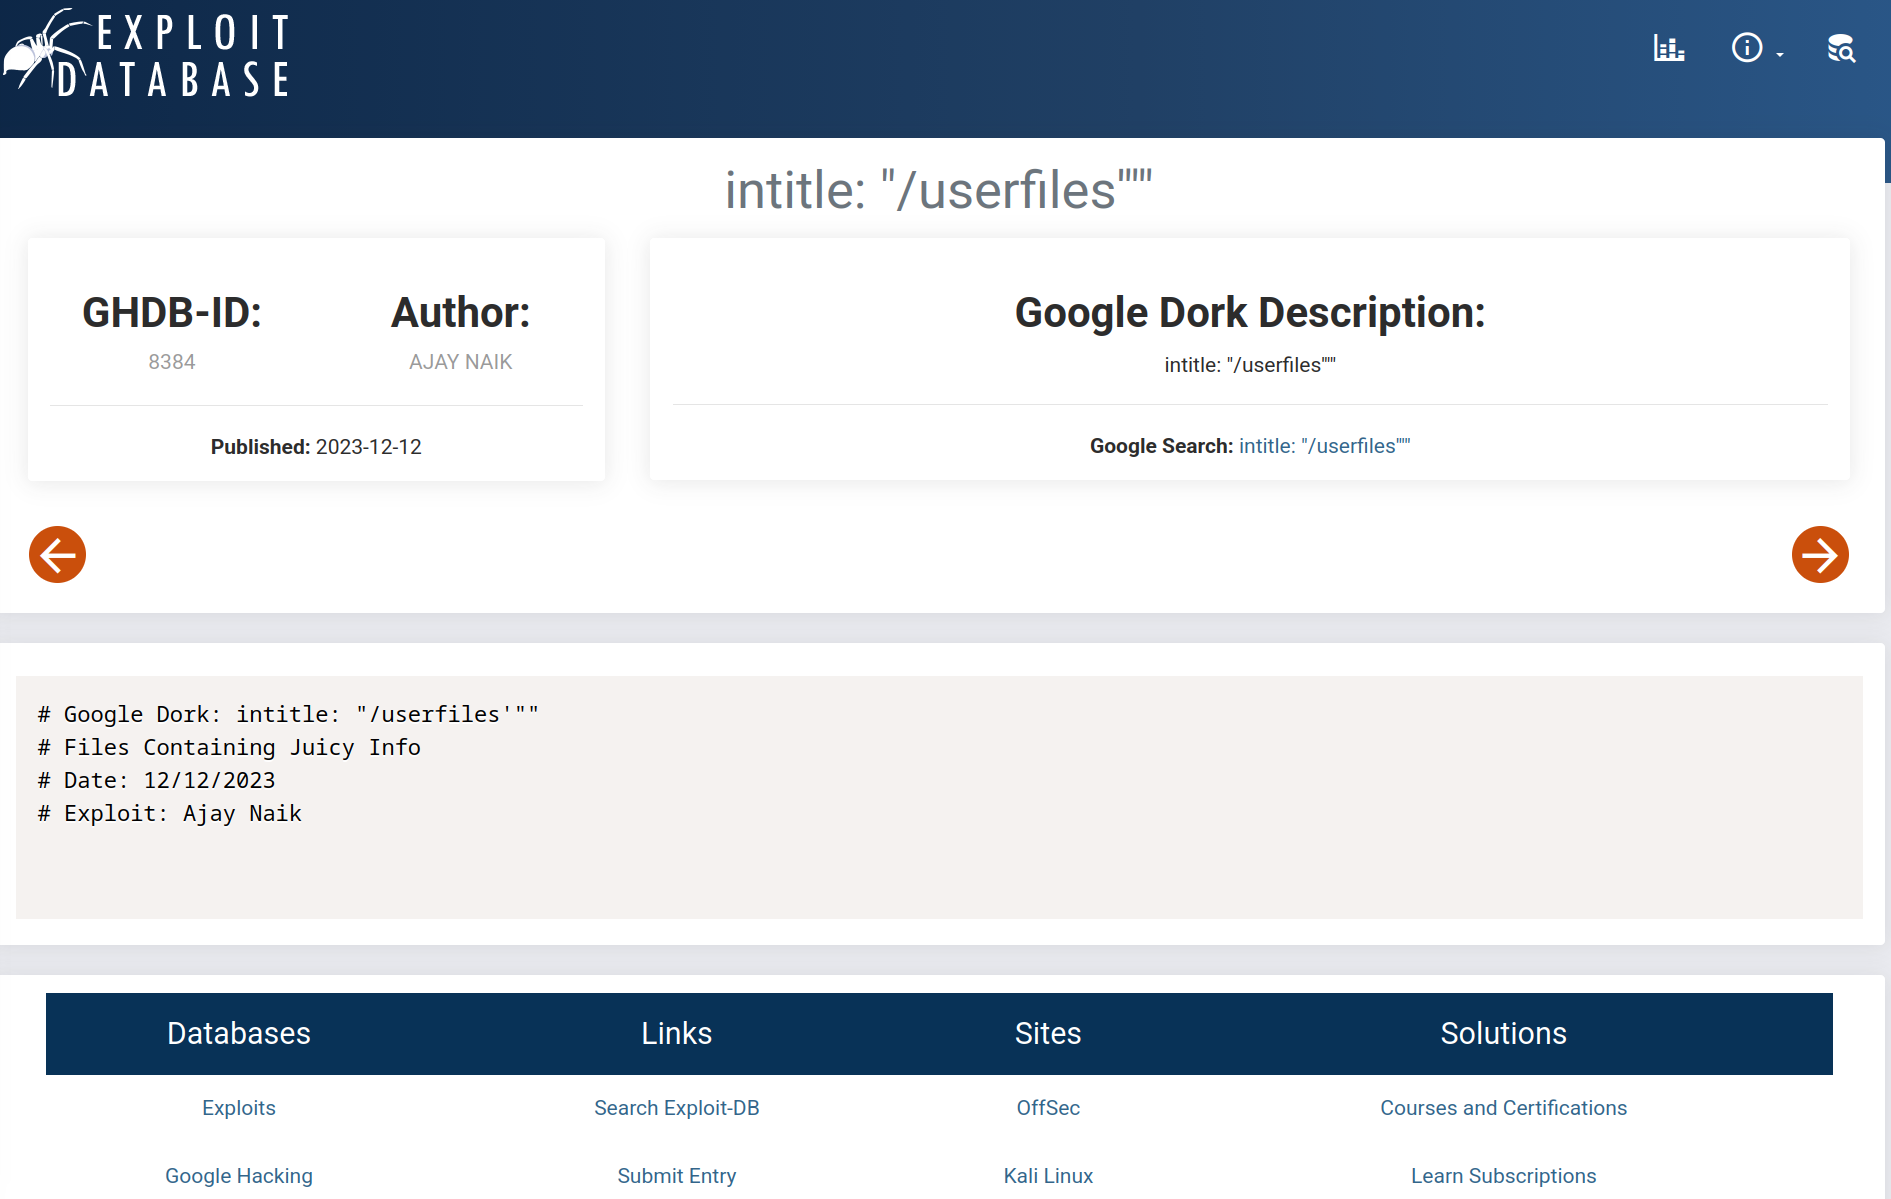
\includegraphics[width=0.95\textwidth]{./fig/atividade4-ghdb.png}
\caption{Google Dork obtido através do Google Hacking Database (GHDB).}
\end{figure}

\subsection{Análise}

\paragraph{}
A consulta busca identificar diretórios expostos na Internet que possam conter
arquivos enviados por usuários, documentos, imagens, backups ou outros dados
armazenados em áreas acessíveis por meio de servidores web.

\paragraph{}
A exposição indevida desse tipo de diretório pode resultar no vazamento de
informações sensíveis, arquivos internos da organização ou documentos que não
deveriam estar disponíveis publicamente.

\paragraph{}
O GHDB demonstra como operadores avançados de busca podem ser utilizados para
identificar recursos expostos na Internet sem a necessidade de interação direta
com os sistemas analisados, constituindo uma importante técnica de
reconhecimento em processos de OSINT.

\paragraph{}
A atividade permitiu compreender a utilização de Google Dorks como ferramenta
de coleta de informações em fontes abertas e a importância de revisar
periodicamente os conteúdos publicados em servidores web para evitar exposição
indevida de informações.
